\documentclass{article}

\usepackage{amsmath}
\usepackage{amssymb}
\usepackage{tikz}
\usetikzlibrary{automata,positioning,arrows}
\tikzset{
	>=stealth',
	initial text=$ $
	}

\title{Assignment 3}
\date{2019-01-31}
\author{MONTGOMERY, BENNET 20074049 CISC223\\
		\and GOEL, CHRISTOPHER 20053408 CISC223\\
		\and DALLAS, SPENCER 20048480 CISC223\\
		\and VIOLO, JARED 20051382 CISC223}

\begin{document}
	\maketitle
	\pagenumbering{arabic}
	
	\section*{Q1.}
	The first thing we need to do is generate the elementary state diagram for $a$:\\\\
	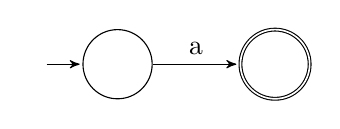
\begin{tikzpicture}[shorten >=1pt,node distance=2cm,on grid,auto] 
   		\node[state,initial] (1) {};  
   		\node[state, accepting] (2) [right=of 1] {};
    	\path[->]
    	(1) edge node {a} (2);
	\end{tikzpicture}
	\\\\Next, we generate the state diagram for $b^*$ and concatenate to $a$ by merging the starting state of $a$ with the starting state of $b^*$. The state diagram of $b^*$ is generated by taking the elementary state diagram of $b$, merging the accepting and starting states, creating a new starting state and connecting it to the previous one via $\epsilon$, and creating a new accepting state and connecting the old accepting state to it via $\epsilon$, giving us the following diagram:\\\\
	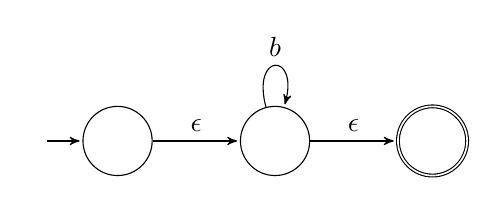
\begin{tikzpicture}[shorten >=1pt,node distance=2cm,on grid, auto]
		\node[state, initial](1) {};
		\node[state] (2) [right=of 1] {};
		\node[state, accepting] (3) [right=of 2] {};
		\path[->]
		(1) edge node {$\epsilon$} (2)
		(2) edge node {$\epsilon$} (3)
			edge [loop above] node {$b$} ();
	\end{tikzpicture}
	\\\\Merging the accepting state of our $a$ diagram with the starting state of $b^*$ gives us :\\\\
	\begin{tikzpicture}[shorten >=1pt,node distance=2cm,on grid,auto] 
   		\node[state,initial] (1) {};  
   		\node[state] (3) [right=of 1] {};
   		\node[state] (4) [right=of 3] {};
   		\node[state,accepting] (5) [right=of 4] {};
    	\path[->]
    	(1) edge node {$a$} (2)
    	(3) edge node {$\epsilon$} (4)
    	(4) edge [loop above] node {$b$} ()
    		edge node {$\epsilon$} (5);
	\end{tikzpicture}
	\\\\Now we need to generate the state transition diagram for $a + c$ and concatenate it to our existing diagram for $ab^*$. We do this by merging the starting and accepting states of the elementary diagrams for $a$ and $c$, giving us the following diagram:\\\\
	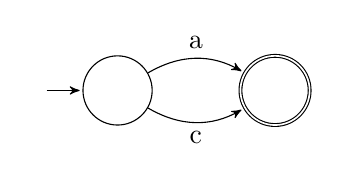
\begin{tikzpicture}[shorten >=1pt,node distance=2cm,on grid,auto]
		\node[state,initial](1){};
		\node[state,accepting] (2) [right=of 1] {};
		\path[->]
		(1) edge [bend left] node {a} (2)
			edge [bend right] node [swap] {c} (2);
	\end{tikzpicture}
	\\\\Concatenating this with our existing diagram gives us: \\\\
	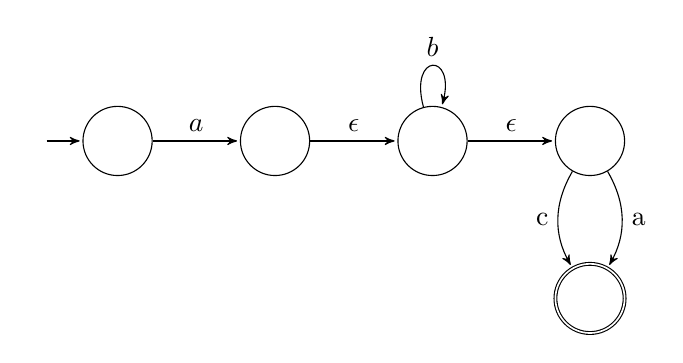
\begin{tikzpicture}[shorten >=1pt,node distance=2cm,on grid,auto] 
   		\node[state,initial] (1) {};  
   		\node[state] (2) [right=of 1] {};
   		\node[state] (4) [right=of 2] {};
   		\node[state] (5) [right=of 4] {};
   		\node[state,accepting] (6) [below=of 5] {};
    	\path[->]
    	(1) edge node {$a$} (2)
    	(2) edge node {$\epsilon$} (4)
    	(4) edge [loop above] node {$b$} ()
    		edge node {$\epsilon$} (5)
  		(5) edge [bend left] node {a} (6)
  			edge [bend right] node [swap] {c} (6);
	\end{tikzpicture}
	\\\\Finally, we need to apply closure to the entire formula. To do this, we merge the accepting state and the starting state. We create a new starting state and link it to the old starting state by an $\epsilon$ transition, and link the old starting state to a new accepting state by a final $\epsilon$ transition. Applying these changes gives us the following unsimplified diagram:\\\\
	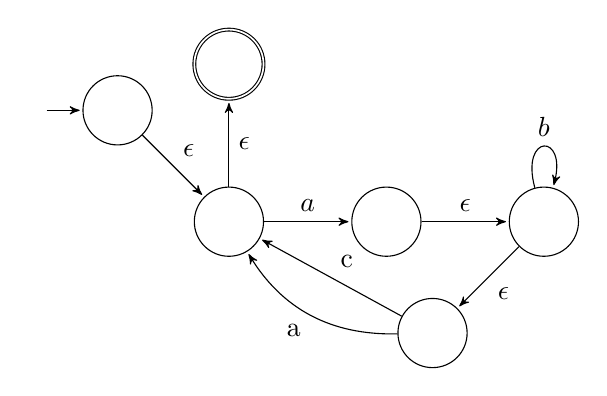
\begin{tikzpicture}[shorten >=1pt,node distance=2cm,on grid,auto] 
   		\node[state] (1) {};  
   		\node[state] (2) [right=of 1] {};
   		\node[state] (4) [right=of 2] {};
   		\node[state] (5) [below left=of 4] {};
   		\node[state,initial] (7) [above left=of 1] {};
   		\node[state,accepting] (8) [above=of 1]{};
    	\path[->]
    	(1) edge node {$a$} (2)
    		edge node [swap] {$\epsilon$} (8)
    	(2) edge node {$\epsilon$} (4)
    	(4) edge [loop above] node {$b$} ()
    		edge node {$\epsilon$} (5)
  		(5) edge [bend left] node {a} (1)
  			edge node [swap] {c} (1)
  		(7) edge node {$\epsilon$} (1);
	\end{tikzpicture}
	\newpage
	\section*{Q2.}
	Since $G$ is the only state that is not the starting or accepting state, it is the only state we need to eliminate. The first thing we need to do is fill in all absent transitions with $\emptyset$ and $\epsilon$ transitions as appropriate:\\\\
	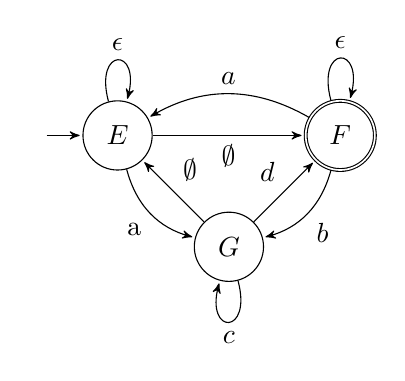
\begin{tikzpicture}[shorten >=1pt,node distance=2cm,on grid,auto] 
		\node[state,initial] (E) {$E$};
		\node[state] (G) [below right=of E] {$G$};
		\node[state,accepting] (F) [above right=of G] {$F$};
		\path[->]
		(E) edge [loop above] node {$\epsilon$} ()
			edge [bend right] node [swap] {a} (G)
			edge node [swap] {$\emptyset$} (F)
		(G) edge node [swap] {$\emptyset$} (E)
			edge node {$d$} (F)
			edge [loop below] node {$c$} ()
		(F) edge [bend right] node [swap] {$a$} (E)
			edge [bend left] node {$b$} (G)
			edge [loop above] node {$\epsilon$} ();
	\end{tikzpicture}
	\\\\In order to eliminate $G$, we need to account for every possible transition chain through $G$ by $E$ and $F$ of at least length 3: we can go from $E$ to $F$ through $G$ with the formula $ac^*d$, we can go from $E$ to $E$ through $G$ with the formula $ac^*\emptyset$, we can go from $F$ to $F$ through $G$ with the formula $bc^*d$, and we can go from $F$ to $E$ through $G$ with the formula $bc^*\emptyset$. Applying all these transitions allow us to eliminate $G$ and produce the following transition state diagram:\\\\
	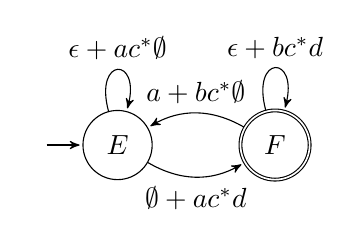
\begin{tikzpicture}[shorten >=1pt,node distance=2cm,on grid,auto] 
		\node[state,initial] (E) {$E$};
		\node[state,accepting] (F) [right=of E] {$F$};
		\path[->]
		(E) edge [loop above] node {$\epsilon + ac^*\emptyset$} ()
			edge [bend right] node [swap] {$\emptyset + ac^*d$} (F)
		(F) edge [bend right] node [swap] {$a + bc^*\emptyset$} (E)
			edge [loop above] node {$\epsilon + bc^*d$} ();
	\end{tikzpicture}
	\\\\We can sub the edge values into the formula $S^*\cdot X\cdot (T + Y \cdot S^* \cdot X)^*$ from the textbook:
		\begin{align*}
			(\epsilon+ac^*\emptyset)^*(\emptyset+ac^*d)((\epsilon+bc^*d) + (a+bc^*\emptyset)(\epsilon+ac^*\emptyset)^*(\emptyset+ac^*d))^*
		\end{align*}
		Applying the facts that $\epsilon$ is the identity for concatenation, $\emptyset$ is the identity for union, and concatenation with $\emptyset$ yields $\emptyset$ the above formula simplifies to:
			\begin{align*}
				&\epsilon^*ac^*d((\epsilon+bc^*d)+a\epsilon^*ac^*d)^*\\
				&=ac^*d((\epsilon+bc^*d)+aac^*d)^*
			\end{align*}
		Which is our final irreducible regular expression.
	\newpage
	\section*{Q3.}
	\subsection*{a)}
	Let $n$ be the number of states in the hypothetical state transition diagram, and let $j = k = m = n$. This makes the formula $a^nb^{n+2}c^{n+1}$. Assuming there exists some string $pqr$ where $pq \neq \epsilon$ and $length(pq) \leq n$. Since $length(pq)\leq n$, $length(q)$ must also be less than $n$, therefore $q$ is some string of $a$ characters. Pumping the $q$ up, eventually we reach a point where the number of $a$ characters in the formula is greater than the number of $c$ characters, that is to say: $j > m+1$. This inequality is not allowed, as $m \geq j$ is clearly stated in the language definition; if we assume the formula is regular, we arrive at a contradiction. Therefore the statement is nonregular.
	\subsection*{(b)}
	The language is defined by the regular expression $aaaaa(aa)^*bbbb^*cc^*+bbbbb^*cc^*d(dd)^*$.
\end{document}